\documentclass[11pt]{article}

\usepackage{fontspec}
\usepackage{graphicx}
\usepackage{xcolor}
\usepackage{array}

\IfFontExistsTF{Microsoft JhengHei}{
  \setmainfont{Microsoft JhengHei}
  \setsansfont{Microsoft JhengHei}
}{
  \setmainfont{Arial}
  \setsansfont{Arial}
}

\special{papersize=24cm,13.5cm}
\setlength{\paperwidth}{24cm}
\setlength{\paperheight}{13.5cm}
\setlength{\textwidth}{21.0cm}
\setlength{\textheight}{12.0cm}
\setlength{\oddsidemargin}{-1.04cm}
\setlength{\evensidemargin}{-1.04cm}
\setlength{\topmargin}{-1.9cm}
\setlength{\headheight}{0cm}
\setlength{\headsep}{0cm}
\setlength{\footskip}{0.2cm}
\pagestyle{empty}
\setlength{\parindent}{0pt}
\setlength{\fboxsep}{7pt}
\setlength{\fboxrule}{0.5pt}

\definecolor{deepblue}{RGB}{28,70,125}
\definecolor{accent}{RGB}{30,125,115}
\definecolor{lightgray}{RGB}{244,246,248}
\definecolor{midgray}{RGB}{95,105,115}

\newcommand{\slidetitle}[1]{%
  {\Large\bfseries\color{deepblue}#1}\par
  \vspace{0.12cm}
  {\color{accent}\rule{\textwidth}{0.8pt}}\par
  \vspace{0.28cm}
}

\newcommand{\card}[1]{%
  \noindent\fcolorbox{lightgray}{lightgray}{%
    \begin{minipage}{\dimexpr\linewidth-2\fboxsep-2\fboxrule-6pt\relax}
    \vspace{0.10cm}
    #1
    \vspace{0.10cm}
    \end{minipage}
  }%
}

\newcommand{\metric}[2]{#1 & \textbf{#2}\\}

\begin{document}

% Slide 1
\vspace*{1.25cm}
\begin{center}
  {\Huge\bfseries\color{deepblue} DSD Final Checkpoint}\par
  \vspace{0.45cm}
  {\Large Baseline checkpoint representation}\par
  \vspace{1.25cm}
  {\Large B12901008 Chung Chia-Yu}\par
  \vfill
  {\color{midgray}May 28, 2026}
\end{center}
\newpage

% Slide 2
\slidetitle{Issues Encountered}
\begin{minipage}[t]{0.47\textwidth}
  \card{
    {\bfseries Reset input delay}\par
    \vspace{0.12cm}
    \small
    The testbench changes reset at a different phase from the memory interface.
    Treating every input with the same delay caused misleading timing pressure
    and gate-level setup messages. The synthesis constraint was updated to use a
    separate reset input delay.
  }
\end{minipage}
\hspace{0.04\textwidth}
\begin{minipage}[t]{0.47\textwidth}
  \card{
    {\bfseries Cache data reset}\par
    \vspace{0.12cm}
    \small
    Cache data arrays do not need to be reset because valid bits define whether a
    line can be used. Removing data-array reset reduced unnecessary reset mux
    paths while keeping valid/dirty/control reset for correctness.
  }
\end{minipage}

\vspace{0.36cm}
\card{
  {\bfseries Current status}\par
  \vspace{0.12cm}
  The baseline processor supports the required checkpoint instruction set,
  handles structural/data/control hazards, includes cache flush support, and
  passes noHazard and hasHazard gate-level simulations at 3.00 ns.
}
\newpage

% Slide 3
\slidetitle{Synthesis Result}
\begin{minipage}[t]{0.47\textwidth}
  \card{
    {\bfseries Timing}\par
    \vspace{0.12cm}
    \begin{tabular}{>{\raggedright\arraybackslash}p{5.55cm}r}
      \metric{Synthesis clock period}{3.00 ns}
      \metric{Worst negative slack}{0.00 ns}
      \metric{Total negative slack}{0.00 ns}
      \metric{Violating paths}{0}
      \metric{Logic levels}{10}
    \end{tabular}
  }

  \vspace{0.28cm}
  \card{
    {\bfseries Gate simulation}\par
    \vspace{0.12cm}
    \begin{tabular}{>{\raggedright\arraybackslash}p{5.55cm}r}
      \metric{Post-syn testbench cycle}{3.00 ns}
      \metric{noHazard sim. time}{1,407,896 ns}
      \metric{hasHazard sim. time}{7,038,896 ns}
    \end{tabular}
  }
\end{minipage}
\hspace{0.04\textwidth}
\begin{minipage}[t]{0.47\textwidth}
  \card{
    {\bfseries Area summary}\par
    \vspace{0.08cm}
    \small
    \begin{tabular}{>{\raggedright\arraybackslash}p{5.35cm}r}
      \metric{Combinational area}{221,357.932724}
      \metric{Buf/Inv area}{34,873.083013}
      \metric{Noncombinational area}{178,868.619936}
      \metric{Macro/Black Box area}{0.000000}
      \metric{Net interconnect area}{3,749,825.752380}
      \metric{Total cell area}{400,226.552660}
      \metric{Total area}{4,150,052.305040}
    \end{tabular}
  }
\end{minipage}
\newpage

% Slide 4
\slidetitle{Gate-Level Simulation}
\begin{minipage}[t]{0.47\textwidth}
  \centering
  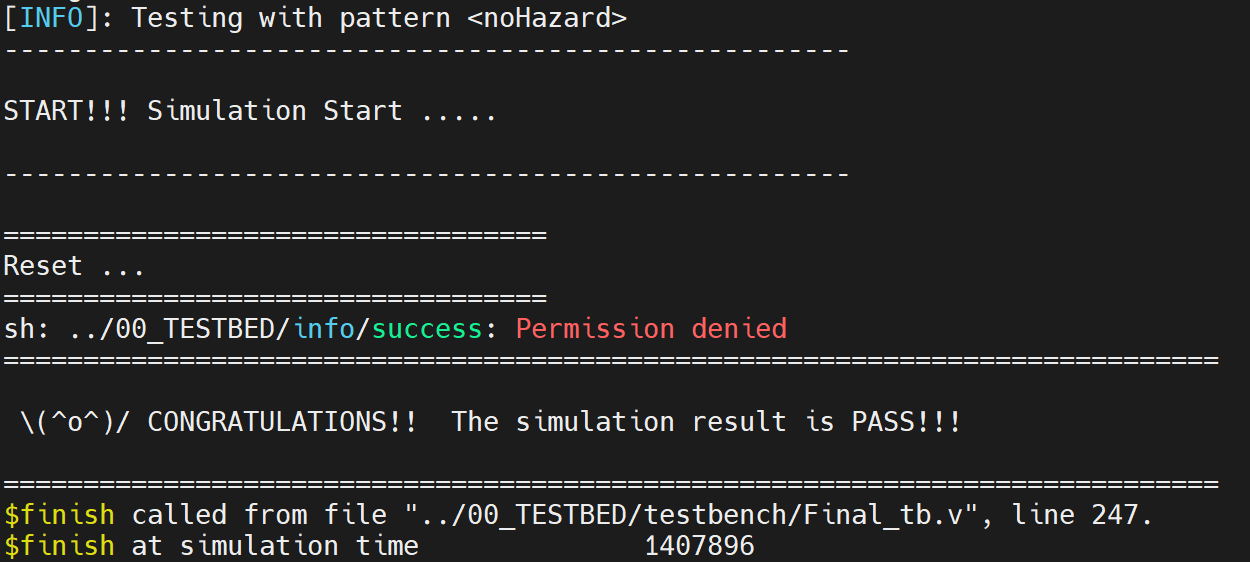
\includegraphics[width=\linewidth,height=5.35cm,keepaspectratio]{no_hazard.png}\par
  \vspace{0.08cm}
  {\small noHazard pattern}
\end{minipage}
\hspace{0.04\textwidth}
\begin{minipage}[t]{0.47\textwidth}
  \centering
  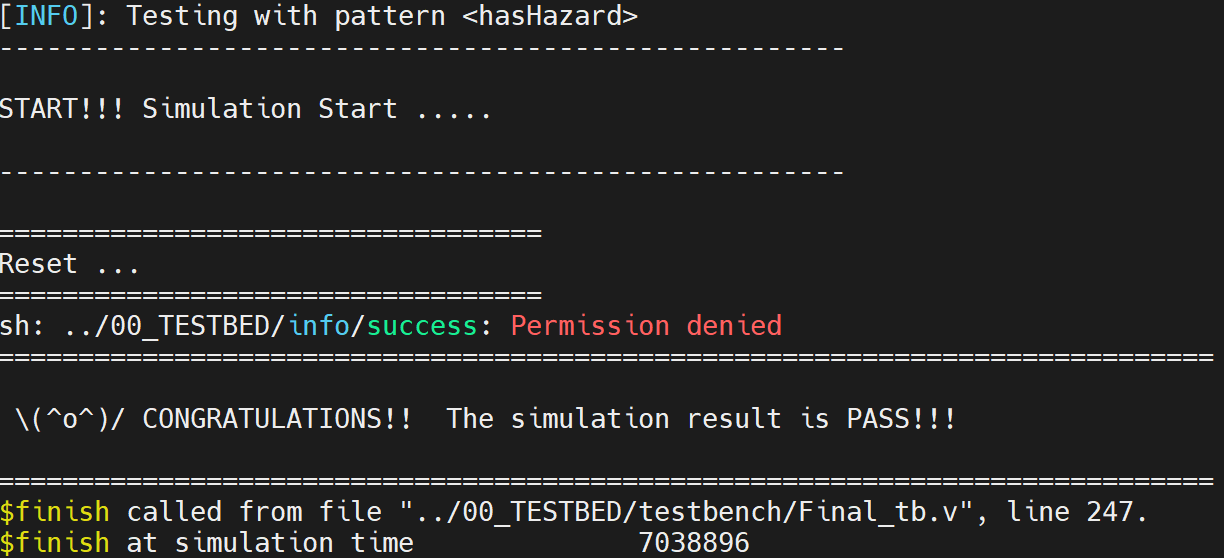
\includegraphics[width=\linewidth,height=5.35cm,keepaspectratio]{has_hazard.png}\par
  \vspace{0.08cm}
  {\small hasHazard pattern}
\end{minipage}

\vspace{0.2cm}
\card{
  Both baseline gate-level simulations pass with SDF annotation at \textbf{3.00 ns}.
}
\newpage

% Slide 5
\slidetitle{Critical Path and Future Plan}
\begin{minipage}[t]{0.52\textwidth}
  \card{
    {\bfseries Cache hit datapath}\par
    \vspace{0.05cm}
    \footnotesize
    \begin{center}
    \begin{tabular}{c}
      \fbox{PC / D-cache address}\\[0.16cm]
      $\downarrow$\\[-0.02cm]
      \fbox{index, tag, word offset decode}\\[0.16cm]
      $\swarrow$ \hspace{1.1cm} $\searrow$\\[-0.02cm]
      \fbox{way0 compare + word select}
      \hspace{0.18cm}
      \fbox{way1 compare + word select}\\[0.16cm]
      $\searrow$ \hspace{1.1cm} $\swarrow$\\[-0.02cm]
      \fbox{hit / way mux}\\[0.16cm]
      $\downarrow$\\[-0.02cm]
      \fbox{pipeline register}
    \end{tabular}
    \end{center}
  }
\end{minipage}
\hspace{0.04\textwidth}
\begin{minipage}[t]{0.40\textwidth}
  \card{
    {\bfseries Observation}\par
    \vspace{0.06cm}
    \small
    Cache access and branch redirection paths are important timing targets for final performance.
  }

  \vspace{0.16cm}
  \card{
    {\bfseries Next steps}\par
    \vspace{0.02cm}
    \small
    \begin{itemize}
      \setlength\itemsep{0.02cm}
      \item Experiment with cache block count and way count.
      \item Tune I-cache/D-cache size and associativity.
      \item Experiment with branch prediction algorithms.
      \item Explore compressed and multiplication extensions.
    \end{itemize}
  }
\end{minipage}

\end{document}
